\documentclass{article}
\usepackage{tikz}
\usepackage{float}
\usepackage{hyperref}

\begin{document}

\title{CSC373 Week 9}
\section{Approximation Algorithms}
\subsection{Vertex Cover}
(From CLRS 35.3)
Given a universe of elements, $E$, and a collection of subsets of $E$, $S=S_1, \ldots , S_n$, find the minimum collection of $S_i$ such that all $E$ are covered (in at least one of the selected $S_i$).

Practice with the following example and come up with an approximation algorithm. What is the worst case approximation relative to the OPT?
\begin{figure}[H]
\centering



\begin{tikzpicture}
	\foreach \x in {0,...,5}{
		\foreach \y in {0,...,2}{
			\node [draw, circle]  (\x\y) at (1.5*\x,1.5*\y) {};
		}
		\draw (1.5*\x -0.25, -0.5) rectangle (1.5*\x + 0.25, 3.5);
		\draw (1.5*\x -0.5, -0.6) rectangle (1.5*\x + 0.5, 0.5);
	}
	\foreach \x in {0,...,1}{
		\draw (\x*4.5-0.5, 2.5) rectangle (\x*4.5 + 3.5, 3.75) 
	}
	\foreach \x in {0,...,2}{
		\draw (\x*3-0.5, 1) rectangle (\x*3 + 2, 2) 
	}


\end{tikzpicture}

\end{figure}

\subsection{Flow}
\href{Previous Problem Set}{https://mcs.utm.utoronto.ca/~zingarod/373/ps/ps5.pdf}. Try out  #1. Here is an example graph to help you get started:

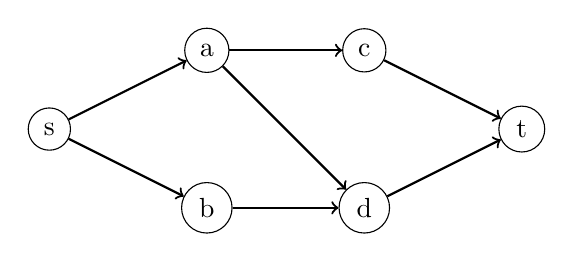
\begin{tikzpicture}
	\node [draw, circle] (s) at (0,0) {s};
	\node [draw, circle] (a) at (2,1) {a};
	\node [draw, circle] (b) at (2,-1) {b};
	\node [draw, circle] (c) at (4,1) {c};
	\node [draw, circle] (d) at (4,-1) {d};
	\node [draw, circle] (t) at (6,0) {t};

	\draw [->, thick] (s) edge node[above] {} (a);
	\draw [->, thick] (s) edge node[above] {} (b);
	\draw [->, thick] (a) edge node[above] {} (c);
	\draw [->, thick] (a) edge node[above] {} (d);
	\draw [->, thick] (b) edge node[above] {} (d);
	\draw [->, thick] (c) edge node[above] {} (t);
	\draw [->, thick] (d) edge node[above] {} (t);
\end{tikzpicture}

\end{document}
